\subsection{El Producto Vectorial de Gibbs (Producto Cruz)}

\subsubsection{Naturaleza y Origen Histórico}

A diferencia del producto escalar, el cual produce un número real, se define una segunda forma de multiplicación vectorial cuyo resultado es un nuevo vector. A esta operación se le denomina \textbf{producto vectorial} o \textbf{producto cruz}. La característica geométrica fundamental del vector resultante es que este es simultáneamente ortogonal a los dos vectores originales que fueron multiplicados.

Históricamente, el producto vectorial moderno fue formulado de manera independiente a finales del siglo XIX por el físico estadounidense Josiah Willard Gibbs y el ingeniero británico Oliver Heaviside. Este operador matemático surge como una extracción y simplificación del álgebra de los cuaterniones (desarrollada previamente por William Rowan Hamilton). Fue diseñado específicamente para facilitar el análisis espacial en áreas como el electromagnetismo y la mecánica clásica.

\subsubsection{Dimensionalidad del Producto Vectorial}

Es importante mencionar una particularidad matemática sobre esta operación. El producto cruz tradicional, entendido como una operación binaria que toma dos vectores y devuelve un tercer vector ortogonal a ambos, es un fenómeno algebraico que está estrictamente definido solo en el espacio tridimensional $\mathbb{R}^3$ (y, de forma excepcional, en $\mathbb{R}^7$). 

No obstante, el concepto de producto vectorial sí existe y es generalizado para vectores en un espacio de $N$ dimensiones ($\mathbb{R}^n$). Esta generalización es formalizada mediante el álgebra exterior (utilizando el producto cuña o \textit{wedge product}, $\wedge$), donde el resultado no es un vector tradicional, sino una entidad matemática de dimensión superior llamada bivector o multivector. 

Sin embargo, para los objetivos y el alcance del cálculo multivariable a este nivel, el estudio del producto vectorial se limitará exclusivamente a la multiplicación de dos vectores en el espacio tridimensional $\mathbb{R}^3$.

\subsubsection{Definición Algebraica en $\mathbb{R}^3$}

El cálculo algebraico del producto cruz se realiza a partir de las componentes rectangulares de los vectores. Se utiliza como herramienta mnemotécnica el cálculo del determinante de una matriz de $3 \times 3$, en cuya primera fila se colocan los vectores unitarios canónicos.

\begin{mydefinition}{Producto Cruz en $\mathbb{R}^3$}
Sean $\vec{u} = (u_1, u_2, u_3)$ y $\vec{v} = (v_1, v_2, v_3)$ dos vectores en $\mathbb{R}^3$. El producto vectorial $\vec{u} \times \vec{v}$ (léase ``$\vec{u}$ cruz $\vec{v}$'') es el vector definido por el siguiente determinante formal:

\[ \vec{u} \times \vec{v} = \begin{vmatrix} 
\hat{\imath} & \hat{\jmath} & \hat{k} \\ 
u_1 & u_2 & u_3 \\ 
v_1 & v_2 & v_3 
\end{vmatrix} \]

Al expandir el determinante por los cofactores de la primera fila, se obtiene la fórmula algebraica:

\[ \vec{u} \times \vec{v} = \begin{vmatrix} u_2 & u_3 \\ v_2 & v_3 \end{vmatrix}\hat{\imath} - \begin{vmatrix} u_1 & u_3 \\ v_1 & v_3 \end{vmatrix}\hat{\jmath} + \begin{vmatrix} u_1 & u_2 \\ v_1 & v_2 \end{vmatrix}\hat{k} \]

\[ \vec{u} \times \vec{v} = (u_2v_3 - u_3v_2)\hat{\imath} - (u_1v_3 - u_3v_1)\hat{\jmath} + (u_1v_2 - u_2v_1)\hat{k} \]
\end{mydefinition}

\subsubsection{Interpretación Geométrica y Regla de la Mano Derecha}

Como se estableció anteriormente, el vector resultante $\vec{u} \times \vec{v}$ es perpendicular tanto al vector $\vec{u}$ como al vector $\vec{v}$. Por consiguiente, es perpendicular al plano que contiene a ambos vectores.

El sentido de este nuevo vector es determinado por la \textbf{Regla de la Mano Derecha}. Si se extienden los dedos de la mano derecha en la dirección del primer vector ($\vec{u}$) y se flexionan hacia el segundo vector ($\vec{v}$), el pulgar extendido indicará la dirección y sentido del vector resultante $\vec{u} \times \vec{v}$. Esta dependencia del orden implica que el producto cruz no es conmutativo, se cumple que $\vec{u} \times \vec{v} = -(\vec{v} \times \vec{u})$.

\begin{center}
\shorthandoff{>}
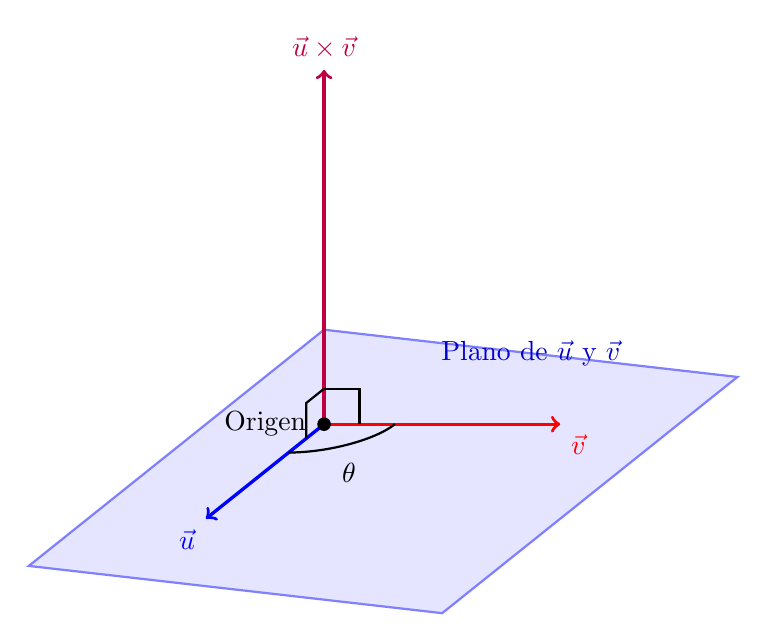
\begin{tikzpicture}[x={(-0.5cm,-0.4cm)}, y={(1cm,0cm)}, z={(0cm,1cm)}, scale=1.5]
    % Plano que contiene a u y v
    \filldraw[fill=blue!10!white, draw=blue!50!white, thick] 
        (-2,-1,0) -- (3,-1,0) -- (4,3,0) -- (-1,3,0) -- cycle;
    \node[blue!80!black] at (-1.5, 1, 0) {Plano de $\vec{u}$ y $\vec{v}$};
    
    % Vectores base u y v
    \draw[->, very thick, blue] (0,0,0) -- (2,0,0) node[below left] {$\vec{u}$};
    \draw[->, very thick, red] (0,0,0) -- (0,2,0) node[below right] {$\vec{v}$};
    
    % Ángulo theta entre u y v
    \draw[thick] (0.6,0,0) arc (0:90:0.6) node[midway, below=3pt] {$\theta$};
    
    % Vector Producto Cruz Resultante
    \draw[->, very thick, purple] (0,0,0) -- (0,0,3) node[above] {$\vec{u} \times \vec{v}$};
    
    % Indicadores de perpendicularidad
    % Con u
    \draw[thick] (0.3,0,0) -- (0.3,0,0.3) -- (0,0,0.3);
    % Con v
    \draw[thick] (0,0.3,0) -- (0,0.3,0.3) -- (0,0,0.3);
    
    % Punto de origen
    \filldraw[black] (0,0,0) circle (1.5pt) node[left=3pt] {Origen};
\end{tikzpicture}
\end{center}

Para verificar que dos vectores son perpendiculares, basta con demostrar que su producto punto es igual a cero. Por lo tanto, si $\vec{w} = \vec{u} \times \vec{v}$, se debe cumplir de manera simultánea que $\vec{w} \cdot \vec{u} = 0$ y $\vec{w} \cdot \vec{v} = 0$.

\begin{proof}[Demostración de Ortogonalidad]
Sean $\vec{u} = (u_1, u_2, u_3)$ y $\vec{v} = (v_1, v_2, v_3)$. A partir de la definición algebraica del producto cruz obtenida por los cofactores, se tiene el vector resultante:
\[
\vec{u} \times \vec{v} = (u_2v_3 - u_3v_2, \, u_3v_1 - u_1v_3, \, u_1v_2 - u_2v_1)
\]

Se evaluará primero el producto punto entre el vector resultante y el vector original $\vec{u}$:
\[
(\vec{u} \times \vec{v}) \cdot \vec{u} = (u_2v_3 - u_3v_2)(u_1) + (u_3v_1 - u_1v_3)(u_2) + (u_1v_2 - u_2v_1)(u_3)
\]

Distribuyendo cada componente de $\vec{u}$ en los binomios correspondientes:
\[
(\vec{u} \times \vec{v}) \cdot \vec{u} = (u_1u_2v_3 - u_1u_3v_2) + (u_2u_3v_1 - u_1u_2v_3) + (u_1u_3v_2 - u_2u_3v_1)
\]

Al eliminar los paréntesis y reorganizar los términos, se observa que todos los componentes se cancelan mutuamente:
\[
(\vec{u} \times \vec{v}) \cdot \vec{u} = u_1u_2v_3 - u_1u_2v_3 - u_1u_3v_2 + u_1u_3v_2 + u_2u_3v_1 - u_2u_3v_1
\]
\[
(\vec{u} \times \vec{v}) \cdot \vec{u} = 0
\]

Este resultado demuestra algebraicamente que el vector $\vec{u} \times \vec{v}$ es perpendicular al vector $\vec{u}$. Realizando el mismo desarrollo para el producto $(\vec{u} \times \vec{v}) \cdot \vec{v}$ resultará también $0$, demostrando que el vector resultante es ortogonal a ambos vectores base de manera simultánea.
\end{proof}

\subsubsection{Propiedades Algebraicas del Producto Vectorial}

Al igual que las otras operaciones vectoriales, el producto cruz posee propiedades matemáticas definidas. Sean $\vec{u}$, $\vec{v}$ y $\vec{w}$ vectores en $\mathbb{R}^3$, y sea $c$ un escalar. Se cumplen las siguientes propiedades:

\begin{mytheorem}{Propiedades del Producto Vectorial}
\begin{enumerate}
    \item \textbf{Anticonmutatividad:} $\vec{u} \times \vec{v} = -(\vec{v} \times \vec{u})$
    \item \textbf{Distributividad sobre la suma:} $\vec{u} \times (\vec{v} + \vec{w}) = (\vec{u} \times \vec{v}) + (\vec{u} \times \vec{w})$
    \item \textbf{Asociatividad escalar:} $c(\vec{u} \times \vec{v}) = (c\vec{u}) \times \vec{v} = \vec{u} \times (c\vec{v})$
    \item \textbf{Producto con el vector cero:} $\vec{u} \times \vec{0} = \vec{0} \times \vec{u} = \vec{0}$
    \item \textbf{Producto consigo mismo:} $\vec{u} \times \vec{u} = \vec{0}$
\end{enumerate}
\end{mytheorem}

\subsubsection{Magnitud del Producto Vectorial}

De manera análoga al producto punto, existe una relación entre la magnitud del producto vectorial y el ángulo $\theta$ que se forma entre los dos vectores originales (donde $0 \leq \theta \leq \pi$). Mientras que el producto punto se relaciona con el coseno del ángulo, la magnitud del producto cruz está directamente vinculada con la función seno.

\begin{mytheorem}{Magnitud del Producto Cruz}
Si $\theta$ es el ángulo entre dos vectores no nulos $\vec{u}$ y $\vec{v}$, entonces la magnitud de su producto cruz es:
\[ \|\vec{u} \times \vec{v}\| = \|\vec{u}\| \|\vec{v}\| \sin(\theta) \]
\end{mytheorem}

\begin{proof}[Demostración]
Sean $\vec{u} = (u_1, u_2, u_3)$ y $\vec{v} = (v_1, v_2, v_3)$. A partir de la definición algebraica del producto cruz, se calcula el cuadrado de su magnitud elevando al cuadrado cada una de sus componentes:
\[ \|\vec{u} \times \vec{v}\|^2 = (u_2v_3 - u_3v_2)^2 + (u_3v_1 - u_1v_3)^2 + (u_1v_2 - u_2v_1)^2 \]

Se desarrollan los tres binomios al cuadrado:
\[ \|\vec{u} \times \vec{v}\|^2 = (u_2v_3 - u_3v_2)^2 + (u_3v_1 - u_1v_3)^2 + (u_1v_2 - u_2v_1)^2 \]

Para agrupar estos términos, se suma y se resta la misma cantidad, específicamente la suma de los cuadrados de los productos de componentes homólogas $(u_1^2v_1^2 + u_2^2v_2^2 + u_3^2v_3^2)$, lo cual no altera el valor de la ecuación:
\[ \quad + u_1^2v_1^2 + u_2^2v_2^2 + u_3^2v_3^2 - (u_1^2v_1^2 + u_2^2v_2^2 + u_3^2v_3^2) \]

Al reorganizar la expresión, se agrupan todos los términos positivos por un lado y los negativos por otro:
\[ \|\vec{u} \times \vec{v}\|^2 = (u_1^2v_1^2 + u_1^2v_2^2 + u_1^2v_3^2 + u_2^2v_1^2 + u_2^2v_2^2 + u_2^2v_3^2 + u_3^2v_1^2 + u_3^2v_2^2 + u_3^2v_3^2) \]
\[ \quad \quad \quad - (u_1^2v_1^2 + u_2^2v_2^2 + u_3^2v_3^2 + 2u_1v_1u_2v_2 + 2u_1v_1u_3v_3 + 2u_2v_2u_3v_3) \]

El primer grupo de términos positivos corresponde exactamente al desarrollo del producto de las magnitudes al cuadrado de los vectores originales. El segundo grupo corresponde al trinomio cuadrado perfecto del producto punto. Por lo tanto, se factoriza la expresión como:
\[ \|\vec{u} \times \vec{v}\|^2 = (u_1^2 + u_2^2 + u_3^2)(v_1^2 + v_2^2 + v_3^2) - (u_1v_1 + u_2v_2 + u_3v_3)^2 \]

Sustituyendo por las definiciones formales de magnitud y producto escalar:
\[ \|\vec{u} \times \vec{v}\|^2 = \|\vec{u}\|^2 \|\vec{v}\|^2 - (\vec{u} \cdot \vec{v})^2 \]

A partir del teorema del producto punto, se sabe que $\vec{u} \cdot \vec{v} = \|\vec{u}\|\|\vec{v}\|\cos(\theta)$. Sustituyendo esta expresión geométrica en la ecuación:
\[ \|\vec{u} \times \vec{v}\|^2 = \|\vec{u}\|^2 \|\vec{v}\|^2 - (\|\vec{u}\|\|\vec{v}\|\cos(\theta))^2 \]

Distribuyendo el exponente cuadrado en el segundo término y factorizando el elemento común $\|\vec{u}\|^2 \|\vec{v}\|^2$:
\[ \|\vec{u} \times \vec{v}\|^2 = \|\vec{u}\|^2 \|\vec{v}\|^2 - \|\vec{u}\|^2\|\vec{v}\|^2\cos^2(\theta) \]
\[ \|\vec{u} \times \vec{v}\|^2 = \|\vec{u}\|^2 \|\vec{v}\|^2 (1 - \cos^2(\theta)) \]

Aplicando la identidad trigonométrica pitagórica fundamental ($1 - \cos^2\theta = \sin^2\theta$):
\[ \|\vec{u} \times \vec{v}\|^2 = \|\vec{u}\|^2 \|\vec{v}\|^2 \sin^2(\theta) \]

Finalmente, al extraer la raíz cuadrada en ambos lados de la ecuación, y considerando que $\sin(\theta) \geq 0$ para ángulos comprendidos entre $0$ y $\pi$ ($0^\circ \leq \theta \leq 180^\circ$), se concluye la demostración:
\[ \|\vec{u} \times \vec{v}\| = \|\vec{u}\| \|\vec{v}\| \sin(\theta) \]
\end{proof}

\subsubsection{Condición de Paralelismo}

Este teorema sobre la magnitud ofrece una herramienta algebraica directa para determinar si dos vectores son paralelos. Si dos vectores no nulos $\vec{u}$ y $\vec{v}$ son paralelos (o colineales), el ángulo entre ellos es exactamente $\theta = 0$ (si apuntan en la misma dirección) o $\theta = \pi$ (si apuntan en direcciones opuestas).

En ambos casos, el seno del ángulo es cero. Sustituyendo este valor en la fórmula de la magnitud:
\[ \|\vec{u} \times \vec{v}\| = \|\vec{u}\| \|\vec{v}\| (0) = 0 \]

Dado que el único vector cuya magnitud es cero es el vector nulo ($\vec{0}$), se deduce el siguiente criterio:

\begin{mytheorem}{Vectores Paralelos}
Dos vectores no nulos $\vec{u}$ y $\vec{v}$ son paralelos si y solo si su producto vectorial es el vector cero:
\[ \vec{u} \times \vec{v} = \vec{0} \]
\end{mytheorem}

\subsection{Productos Triples}

En el análisis vectorial y sus aplicaciones físicas, es frecuente encontrarse con operaciones que involucran tres vectores simultáneamente. Existen dos formas principales de combinar tres vectores utilizando los productos escalar y vectorial: el triple producto escalar y el triple producto vectorial.

\subsubsection{El Triple Producto Escalar}

El triple producto escalar es una operación que toma tres vectores en $\mathbb{R}^3$ y produce un único número real. Se define combinando un producto vectorial seguido de un producto escalar.

\begin{mydefinition}{Triple Producto Escalar}
Sean $\vec{u}$, $\vec{v}$ y $\vec{w}$ tres vectores en el espacio tridimensional. El triple producto escalar se define como:
\[ \vec{u} \cdot (\vec{v} \times \vec{w}) \]
\end{mydefinition}

Algebraicamente, esta operación puede ser calculada de manera directa mediante el cálculo del determinante de una matriz de $3 \times 3$ formada por las componentes de los tres vectores. Si $\vec{u} = (u_1, u_2, u_3)$, $\vec{v} = (v_1, v_2, v_3)$ y $\vec{w} = (w_1, w_2, w_3)$, entonces:

\[ \vec{u} \cdot (\vec{v} \times \vec{w}) = \begin{vmatrix} 
u_1 & u_2 & u_3 \\ 
v_1 & v_2 & v_3 \\ 
w_1 & w_2 & w_3 
\end{vmatrix} \]

Una propiedad algebraica del triple producto escalar es que los operadores de punto y cruz pueden intercambiarse sin alterar el resultado, siempre y cuando se mantenga el orden de los vectores. Es decir, se cumple que $\vec{u} \cdot (\vec{v} \times \vec{w}) = (\vec{u} \times \vec{v}) \cdot \vec{w}$.

\subsubsection{El Triple Producto Vectorial}

A diferencia del caso anterior, el triple producto vectorial es una operación que devuelve como resultado un nuevo vector en el espacio. Se obtiene al realizar el producto cruz de un vector con el resultado de un producto cruz previo.

\begin{mydefinition}{Triple Producto Vectorial}
Sean $\vec{u}$, $\vec{v}$ y $\vec{w}$ tres vectores en $\mathbb{R}^3$. El triple producto vectorial se denota formalmente como:
\[ \vec{u} \times (\vec{v} \times \vec{w}) \]
\end{mydefinition}

Es crucial recalcar que, debido a que el producto vectorial no goza de la propiedad asociativa, la colocación de los paréntesis es estrictamente obligatoria, pues se cumple que $\vec{u} \times (\vec{v} \times \vec{w}) \neq (\vec{u} \times \vec{v}) \times \vec{w}$.

Desde un análisis geométrico, el vector resultante de $\vec{u} \times (\vec{v} \times \vec{w})$ yace exactamente en el mismo plano que está siendo formado por los vectores $\vec{v}$ y $\vec{w}$. Esto se debe a que el resultado de la operación debe ser ortogonal al vector $(\vec{v} \times \vec{w})$, y dado que este último es ortogonal al plano de $\vec{v}$ y $\vec{w}$, el vector final se ve forzado a existir dentro de dicho plano inicial.

\paragraph{Regla de BAC-CAB}
Para calcular este producto sin necesidad de evaluar dos determinantes matrices de forma consecutiva, se emplea una identidad matemática conocida como la Fórmula de Expulsión o regla BAC-CAB. Esta identidad permite expresar el vector resultante de forma mucho más directa, como una combinación lineal de los vectores $\vec{v}$ y $\vec{w}$, utilizando únicamente operaciones de producto punto y escalado:

\begin{mytheorem}{Identidad del Triple Producto Vectorial}
\[ \vec{u} \times (\vec{v} \times \vec{w}) = \vec{v}(\vec{u} \cdot \vec{w}) - \vec{w}(\vec{u} \cdot \vec{v}) \]
\end{mytheorem}

\paragraph{Demostración mediante Notación Tensorial}

La demostración analítica tradicional de la regla BAC-CAB mediante el cálculo de determinantes resulta en un proceso algebraico sumamente extenso y propenso a errores. Para simplificar esta demostración, se emplea la notación tensorial.

Antes de proceder con la demostración, es necesario definir dos operadores fundamentales en esta notación:

\begin{enumerate}
    \item \textbf{La Delta de Kronecker ($\delta_{ij}$):} Es un operador que vale $1$ si los índices son iguales ($i = j$) y $0$ si son diferentes ($i \neq j$). Al multiplicar un vector por la delta de Kronecker, ocurre un fenómeno llamado contracción de índices, que simplemente renombra el índice: $\delta_{ij}v_j = v_i$. Además, el producto punto se define como: $\vec{u} \cdot \vec{v} = u_i v_i$.
    \item \textbf{El Símbolo de Levi-Civita ($\epsilon_{ijk}$):} Es un tensor alternante que vale $1$ si los índices $(i,j,k)$ son una permutación cíclica de $(1,2,3)$, vale $-1$ si es una permutación anticíclica, y vale $0$ si algún índice se repite. Su utilidad principal es definir el producto cruz en su $i$-ésima componente: 
    \[ (\vec{u} \times \vec{v})_i = \epsilon_{ijk} u_j v_k \]
\end{enumerate}

El elemento clave para esta demostración es una identidad matemática que relaciona el producto de dos símbolos de Levi-Civita con deltas de Kronecker, conocida como la identidad epsilon-delta:
\[ \epsilon_{ijk} \epsilon_{klm} = \epsilon_{kij} \epsilon_{klm} = \delta_{il}\delta_{jm} - \delta_{im}\delta_{jl} \]

Con estas herramientas, se procede a la demostración del teorema.

\begin{proof}[Demostración de la Regla BAC-CAB]
Sea el vector resultante $\vec{R} = \vec{u} \times (\vec{v} \times \vec{w})$. Se buscará aislar la $i$-ésima componente de este vector, es decir, $R_i$.

\textbf{Paso 1: Aplicación del primer producto cruz.}
Se aplica la definición tensorial del producto cruz al operador externo, asignando los índices $i, j, k$:
\[ R_i = [\vec{u} \times (\vec{v} \times \vec{w})]_i = \epsilon_{ijk} u_j (\vec{v} \times \vec{w})_k \]
\textbf{Paso 2: Aplicación del segundo producto cruz.}
Ahora se aplica la misma definición para el producto cruz interno, cuya componente es $k$. Para evitar confusión, se utilizan nuevos índices $l, m$ para los vectores internos:
\[ (\vec{v} \times \vec{w})_k = \epsilon_{klm} v_l w_m \]

\textbf{Paso 3: Sustitución y reordenamiento.}
Se sustituye el resultado del paso 2 en la ecuación del paso 1. Como los escalares conmutan, se agrupan los símbolos de Levi-Civita al inicio de la expresión:
\[ R_i = \epsilon_{ijk} u_j (\epsilon_{klm} v_l w_m) = \epsilon_{ijk} \epsilon_{klm} u_j v_l w_m \]

Debido a que el símbolo de Levi-Civita permite permutaciones cíclicas sin alterar su signo ($\epsilon_{ijk} = \epsilon_{kij}$), se reescribe el primer símbolo para preparar la aplicación de la identidad:
\[ R_i = \epsilon_{kij} \epsilon_{klm} u_j v_l w_m \]

\textbf{Paso 4: Aplicación de la identidad epsilon-delta.}
Se sustituye el producto de los tensores de Levi-Civita por la identidad de deltas de Kronecker ($\epsilon_{kij} \epsilon_{klm} = \delta_{il}\delta_{jm} - \delta_{im}\delta_{jl}$):
\[ R_i = (\delta_{il}\delta_{jm} - \delta_{im}\delta_{jl}) u_j v_l w_m \]

\textbf{Paso 5: Distribución algebraica.}
Se distribuyen los componentes vectoriales dentro del paréntesis:
\[ R_i = (\delta_{il}\delta_{jm} u_j v_l w_m) - (\delta_{im}\delta_{jl} u_j v_l w_m) \]

\textbf{Paso 6: Contracción de índices.}
Se aplica la propiedad de la delta de Kronecker para colapsar los índices. 
En el primer término:
\begin{itemize}
    \item $\delta_{il} v_l$ transforma el índice $l$ en $i$, resultando en $v_i$.
    \item $\delta_{jm} u_j w_m$ filtra las componentes donde $j = m$, resultando en $u_j w_j$.
\end{itemize}
En el segundo término:
\begin{itemize}
    \item $\delta_{im} w_m$ transforma el índice $m$ en $i$, resultando en $w_i$.
    \item $\delta_{jl} u_j v_l$ filtra las componentes donde $j = l$, resultando en $u_j v_j$.
\end{itemize}

Sustituyendo estas contracciones en la ecuación:
\[ R_i = v_i (u_j w_j) - w_i (u_j v_j) \]

\textbf{Paso 7: Conversión a notación vectorial estándar.}
Se reconoce que los términos con índices repetidos ($u_j w_j$ y $u_j v_j$) corresponden a la definición del producto escalar (producto punto). Por lo tanto:
\[ R_i = v_i (\vec{u} \cdot \vec{w}) - w_i (\vec{u} \cdot \vec{v}) \]

Dado que esta igualdad se cumple para cualquier componente $i$ arbitraria, se generaliza para todo el vector, concluyendo así la demostración matemática:
\[ \vec{R} = \vec{v} (\vec{u} \cdot \vec{w}) - \vec{w} (\vec{u} \cdot \vec{v}) \]
\end{proof}

\subsection{Aplicaciones geométricas}

El producto cruz tiene dos aplicaciones geométricas importantes: el cálculo de áreas y el cálculo de volúmenes. En ambos casos, la magnitud del producto cruz se relaciona directamente con la medida geométrica que se desea calcular.

\subsubsection{Área de un paralelogramo}

Una de las aplicaciones geométricas del producto vectorial radica en su capacidad para calcular áreas en el espacio tridimensional. Específicamente, se establece que la magnitud del producto cruz de dos vectores es igual al área del paralelogramo que estos forman cuando se sitúan con un origen común.

Para comprender el origen de esta propiedad, es necesario recurrir a la geometría euclidiana clásica. El área de cualquier paralelogramo se calcula mediante el producto de la longitud de su base por su altura perpendicular:
\[ \text{Área} = (\text{base}) \times (\text{altura}) \]

Supóngase que se tienen dos vectores no nulos $\vec{u}$ y $\vec{v}$ separados por un ángulo $\theta$. Si estos vectores se utilizan para definir los lados adyacentes de un paralelogramo, se puede realizar la siguiente deducción geométrica:

\begin{enumerate}
    \item \textbf{La base:} Se define arbitrariamente al vector $\vec{u}$ como la base de la figura. Por lo tanto, la longitud de la base es exactamente la magnitud de este vector: $\text{base} = \|\vec{u}\|$.
    \item \textbf{La altura ($h$):} La altura del paralelogramo es la distancia perpendicular trazada desde la punta del vector $\vec{v}$ hasta la línea de acción del vector $\vec{u}$. Esto forma un triángulo rectángulo donde la hipotenusa es la magnitud de $\vec{v}$ ($\|\vec{v}\|$). Utilizando la definición de la función seno, se despeja la altura:
    \[ h = \|\vec{v}\| \sin(\theta) \]
\end{enumerate}

Al sustituir estos dos componentes en la fórmula geométrica del área, se obtiene:
\[ \text{Área} = \|\vec{u}\| (\|\vec{v}\| \sin\theta) \]

Como se demostró anteriormente, la expresión $\|\vec{u}\| \|\vec{v}\| \sin\theta$ corresponde a la magnitud del producto cruz entre dichos vectores. Por consiguiente, se tiene el siguiente teorema:

\begin{mytheorem}{Área del Paralelogramo}
El área $A$ del paralelogramo definido por los vectores adyacentes $\vec{u}$ y $\vec{v}$ está dada por la magnitud de su producto vectorial:
\[ A = \|\vec{u} \times \vec{v}\| \]
\end{mytheorem}

\begin{center}
\shorthandoff{>}
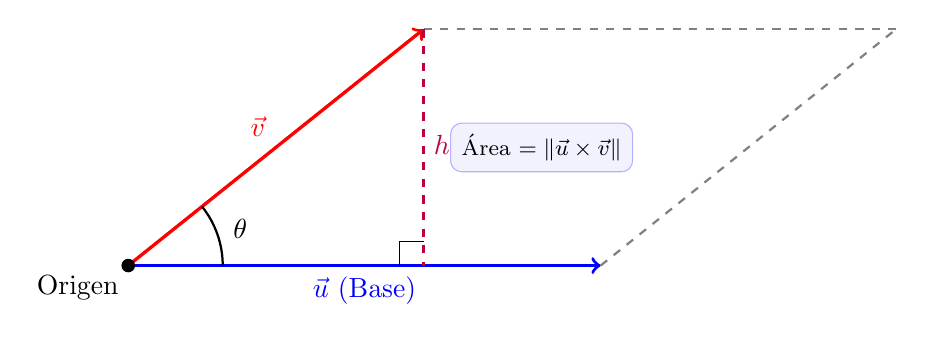
\begin{tikzpicture}[scale=1.5]
    % Base vector u
    \draw[->, very thick, blue] (0,0) -- (4,0) node[midway, below] {$\vec{u}$ (Base)};

    % Vector v
    \draw[->, very thick, red] (0,0) -- (2.5,2) node[midway, above left] {$\vec{v}$};

    % Completando el paralelogramo (líneas punteadas)
    \draw[dashed, thick, gray] (4,0) -- (6.5,2);
    \draw[dashed, thick, gray] (2.5,2) -- (6.5,2);

    % Altura h
    \draw[dashed, thick, purple] (2.5,2) -- (2.5,0) node[midway, right] {$h = \|\vec{v}\|\sin\theta$};

    % Símbolo de ángulo recto para la altura
    \draw (2.3,0) -- (2.3,0.2) -- (2.5,0.2);

    % Ángulo theta
    \draw[thick] (0.8,0) arc (0:38.6:0.8) node[midway, right=2pt, yshift=2pt] {$\theta$};

    % Etiqueta del Área
    \node[font=\footnotesize, fill=blue!5!white, draw=blue!30!white, rounded corners, inner sep=4pt] 
        at (3.5,1) {Área $= \|\vec{u} \times \vec{v}\|$};
        
    % Punto de origen
    \filldraw[black] (0,0) circle (1.5pt) node[below left] {Origen};
\end{tikzpicture}
\end{center}

\paragraph{Corolario: Área de un Triángulo}
Una consecuencia inmediata de este teorema es su aplicación para encontrar el área de un triángulo en el espacio tridimensional. Dado que cualquier paralelogramo puede ser dividido en dos triángulos congruentes trazando una diagonal desde el origen hasta el vértice opuesto, el área del triángulo formado por los vectores $\vec{u}$ y $\vec{v}$ es exactamente la mitad del área del paralelogramo:
\[ \text{Área del triángulo} = \frac{1}{2} \|\vec{u} \times \vec{v}\| \]

\subsubsection{Volúmen de un paralelepípedo}

Mientras que la magnitud del producto cruz simple ($\|\vec{v} \times \vec{w}\|$) proporciona el área de un paralelogramo bidimensional, el triple producto escalar añade una tercera dimensión al cálculo. El valor absoluto de esta operación representa geométricamente el volumen del paralelepípedo tridimensional que se forma al considerar a los tres vectores como aristas adyacentes que comparten un mismo origen.

La justificación geométrica de esto radica en la fórmula del volumen de un prisma. 
\begin{itemize}
    \item El área de la base, conformada por los vectores $\vec{v}$ y $\vec{w}$, está dada por $\|\vec{v} \times \vec{w}\|$.
    \item La altura $h$ del sólido corresponde a la componente del vector $\vec{u}$ sobre el eje ortogonal a la base. Esta altura es igual a $\|\vec{u}\||\cos\theta|$, donde $\theta$ es el ángulo entre $\vec{u}$ y el vector resultante de $\vec{v} \times \vec{w}$.
\end{itemize}

Por lo tanto, al multiplicar la base por la altura, se recupera exactamente la definición del producto punto:
\[ \text{Volumen} = \|\vec{v} \times \vec{w}\| (\|\vec{u}\| |\cos\theta|) = |\vec{u} \cdot (\vec{v} \times \vec{w})| \]

\begin{center}
\shorthandoff{>}
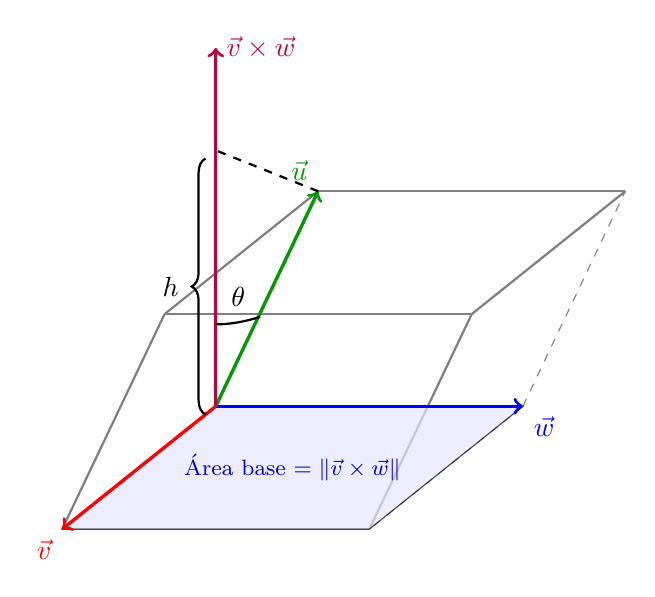
\begin{tikzpicture}[x={(-0.5cm,-0.4cm)}, y={(1cm,0cm)}, z={(0cm,1cm)}, scale=1.3]
    % Vectores base (Base del paralelepipedo)
    \coordinate (O) at (0,0,0);
    \coordinate (V) at (3,0,0);
    \coordinate (W) at (0,3,0);
    \coordinate (U) at (1,1.5,2.5);
    
    % Vértices superiores del paralelepipedo
    \coordinate (VU) at (4,1.5,2.5);
    \coordinate (WU) at (1,4.5,2.5);
    \coordinate (VW) at (3,3,0);
    \coordinate (VWU) at (4,4.5,2.5);
    
    % Dibujo de las aristas ocultas (dashed)
    \draw[dashed, gray] (O) -- (W);
    \draw[dashed, gray] (W) -- (VW);
    \draw[dashed, gray] (W) -- (WU);
    
    % Dibujo de las aristas visibles
    \draw[thick, gray] (V) -- (VW);
    \draw[thick, gray] (U) -- (VU);
    \draw[thick, gray] (U) -- (WU);
    \draw[thick, gray] (VU) -- (VWU);
    \draw[thick, gray] (WU) -- (VWU);
    \draw[thick, gray] (V) -- (VU);
    \draw[thick, gray] (VW) -- (VWU);
    
    % Relleno tenue de la base (paralelogramo)
    \filldraw[fill=blue!10!white, opacity=0.7] (O) -- (V) -- (VW) -- (W) -- cycle;
    \node[blue!80!black, font=\footnotesize] at (1.5, 1.5, 0) {Área base $= \|\vec{v} \times \vec{w}\|$};
    
    % Vectores principales
    \draw[->, very thick, red] (O) -- (V) node[below left] {$\vec{v}$};
    \draw[->, very thick, blue] (O) -- (W) node[below right] {$\vec{w}$};
    \draw[->, very thick, green!60!black] (O) -- (U) node[above left] {$\vec{u}$};
    
    % Vector Producto Cruz (Normal a la base)
    \coordinate (Nx) at (0,0,3.5);
    \draw[->, very thick, purple] (O) -- (Nx) node[right] {$\vec{v} \times \vec{w}$};
    
    % Proyección de u sobre el vector normal (Altura h)
    \draw[dashed, thick, black] (U) -- (0,0,2.5);
    \draw[decorate, decoration={brace, amplitude=5pt}, thick] (0.2,0,0) -- (0.2,0,2.5) node[midway, left=6pt] {$h$};
    
    % Ángulo theta
    \draw[thick] (0,0,0.8) arc (0:58:0.4) node[midway, above=2pt] {$\theta$};
\end{tikzpicture}
\end{center}

\subsection{Ejercicios}

\begin{enumerate}
    \item Calcular el producto cruz $\vec{u} \times \vec{v}$ para cada par de vectores:
\begin{enumerate}
    \item $\vec{u} = (1, 2, 3)$ y $\vec{v} = (4, 5, 6)$
    \item $\vec{u} = (2, -1, 3)$ y $\vec{v} = (0, 4, -2)$
\end{enumerate}
    \item Sean $\vec{u} = (3, -1, 2)$ y $\vec{v} = (1, 4, -1)$. Calcular $\vec{u} \times \vec{v}$ y $\vec{v} \times \vec{u}$. Verificar que $\vec{u} \times \vec{v} = -(\vec{v} \times \vec{u})$.
    \item Sean $\vec{u} = (2, 1, -3)$ y $\vec{v} = (-1, 3, 2)$. Calcular $\vec{w} = \vec{u} \times \vec{v}$ y verificar algebraicamente que $\vec{w}$ es ortogonal tanto a $\vec{u}$ como a $\vec{v}$, es decir, que $\vec{w} \cdot \vec{u} = 0$ y $\vec{w} \cdot \vec{v} = 0$.
    \item Determinar, usando el producto cruz, si los siguientes pares de vectores son paralelos:
\begin{enumerate}
    \item $\vec{u} = (2, -4, 6)$ y $\vec{v} = (-1, 2, -3)$
    \item $\vec{a} = (1, 2, 3)$ y $\vec{b} = (2, 5, 3)$
\end{enumerate}
    \item Sean $\vec{u} = (1, 2, 2)$ y $\vec{v} = (3, 0, 4)$. Usando la relación $\|\vec{u} \times \vec{v}\| = \|\vec{u}\|\|\vec{v}\|\sin\theta$, encontrar el ángulo $\theta$ (en grados) entre los dos vectores. Comparar el resultado obtenido usando la relación análoga con el producto punto.
    \item Encontrar el valor del parámetro $k$ tal que los vectores $\vec{u} = (1, k, 2)$ y $\vec{v} = (3, 1, k)$ sean paralelos.
    \item Calcular el área del paralelogramo y del triángulo formados por los vectores $\vec{u} = (3, -1, 4)$ y $\vec{v} = (2, 2, -1)$ cuando se sitúan con un origen común.
    \item Dados los tres puntos $A = (1, 0, 2)$, $B = (3, 1, 0)$ y $C = (0, 2, 1)$ en $\mathbb{R}^3$:
\begin{enumerate}
    \item Encontrar los vectores $\overrightarrow{AB}$ y $\overrightarrow{AC}$.
    \item Calcular el área del triángulo $ABC$.
\end{enumerate}
    \item Sean $\vec{u} = (1, 0, 2)$, $\vec{v} = (-1, 3, 1)$ y $\vec{w} = (2, 1, -1)$.
\begin{enumerate}
    \item Calcular el triple producto escalar $\vec{u} \cdot (\vec{v} \times \vec{w})$ usando el determinante $3\times 3$.
    \item Verificar que $\vec{u} \cdot (\vec{v} \times \vec{w}) = (\vec{u} \times \vec{v}) \cdot \vec{w}$.
    \item Interpretar geométricamente el resultado: ¿cuál es el volumen del paralelepípedo que forman los tres vectores?
\end{enumerate}
    \item Sean $\vec{u} = (2, 0, 1)$, $\vec{v} = (1, -1, 2)$ y $\vec{w} = (3, 1, 0)$. Verificar la regla BAC-CAB calculando ambos lados de la identidad para el triple producto vectorial:
\[ \vec{u} \times (\vec{v} \times \vec{w}) = \vec{v}(\vec{u} \cdot \vec{w}) - \vec{w}(\vec{u} \cdot \vec{v}) \]
    \item Una llave ejerce una fuerza $\vec{F} = (0, -20, 0)$ N sobre una tuerca ubicada en el punto $Q = (0.3, 0, 0)$ m respecto al punto de pivote $P$ (en metros). El torque mecánico es el producto cruz $\vec{\tau} = \overrightarrow{PQ} \times \vec{F}$.
\begin{enumerate}
    \item Calcular el vector de torque $\vec{\tau}$.
    \item Determinar la magnitud del torque en N$\cdot$m.
    \item Describir la dirección de rotación que produce el torque usando la regla de la mano derecha.
\end{enumerate}
    \item Dados los cuatro vértices de un tetraedro $A = (0,0,0)$, $B = (2,0,0)$, $C = (1,2,0)$ y $D = (1,1,2)$:
\begin{enumerate}
    \item Encontrar los vectores $\overrightarrow{AB}$, $\overrightarrow{AC}$ y $\overrightarrow{AD}$.
    \item Calcular el volumen del paralelepípedo definido por estos tres vectores usando el triple producto escalar.
    \item Sabiendo que el volumen de un tetraedro es $\frac{1}{6}$ del volumen del paralelepípedo que lo contiene, calcular el volumen del tetraedro $ABCD$.
\end{enumerate}
\end{enumerate}